\documentclass[10pt]{article}
\usepackage{times}
\usepackage{fullpage}
\usepackage{fancybox}  % Must include fancybox *before* fancyvrb;
\usepackage{fancyvrb}  % don't know why.
\usepackage[pdftex]{graphicx}
\usepackage{url}
%\usepackage[backref,colorlinks]{hyperref}
\usepackage[authoryear]{natbib}
\usepackage{blindtext}
\usepackage{scrextend}

\setcounter{secnumdepth}{1}
\newcommand{\rscape}{R-scape}

\newcommand{\subtitle}[1]{\newcommand{\plainsubtitle}{#1}}
\newcommand{\subauthor}[1]{\newcommand{\plainsubauthor}{#1}}
\newcommand{\pkgurl}[1]{\newcommand{\plainpkgurl}{#1}}
\newcommand{\pkgversion}[1]{\newcommand{\plainpkgversion}{#1}}
\newcommand{\pkgdate}[1]{\newcommand{\plainpkgdate}{#1}}

% customizations used in the User's Guide


% Description-like environment for documenting functions/APIs.
% puts the description label in a minipage with a large hanging
% indent.
% Good christ this took a long time to develop.
% hanging indent trick stolen from Peter Wilson's hanging.sty @CTAN
% minipage allows multi-line label, and puts item on next line.
% customized list inspired by Kopka/Daly _Guide to LaTeX_ p.213
% SRE, Wed Dec 27 11:37:18 2000
%
\newenvironment{sreapi}{%
     \begin{list}{}{%
       \renewcommand{\makelabel}[1]{%
         \begin{minipage}{\textwidth}%
           \hangindent10em\hangafter1\noindent%
           {\bfseries\texttt{##1}\vspace{0.8em}}%
         \end{minipage}%
     }}}%
     {\end{list}}


% Description-like environment for producing lists like:
%
%     label  stuff, stuff, stuff
%
%    label2  more stuff, more stuff,
%            more stuff.
% \begin{sreitems}{Longest label} \item[label] stuff, ... \end{sreitems}
% SRE, Wed Dec 27 11:59:43 2000
%
\newenvironment{sreitems}[1]{%
     \begin{list}{}{%
       \settowidth{\labelwidth}{#1}%
       \setlength{\leftmargin}{\labelwidth}%
       \addtolength{\leftmargin}{\labelsep}%
       }}
     {\end{list}}
       
\DefineVerbatimEnvironment{sreoutput}{Verbatim}{fontsize=\scriptsize,xleftmargin=2.0\parindent}%
\DefineVerbatimEnvironment{tinysreoutput}{Verbatim}{fontsize=\tiny,xleftmargin=2.0\parindent}%

\makeatletter
\newcommand{\listoffaqs}{\@starttoc{faq}}
\newenvironment{srefaq}[1]
{\addcontentsline{faq}{faq}{#1}\begin{sloppypar}\noindent\slshape\small\begin{quote}\textbf{$\triangleright$ #1}}
{\end{quote}\end{sloppypar}}
\newcommand{\l@faq}[2]{\@dottedtocline{0}{0pt}{0pt}{#1}{#2}}
\makeatother

% Consistent font styles
%   \software{} for the name of a software package
%   \database{} for the name of a database
%   \prog{}     for a program or file name
%   \emprog{}   for an emphasized program or file name
%   \user{}     for a typed user command
%   \response{} for an output line following a \user command
%   \ccode{}    for an inlined C code phrase
\newcommand{\software}[1]{\textsc{#1}}
\newcommand{\database}[1]{\textsc{#1}}
\newcommand{\prog}[1]{{\small\texttt{#1}}}
\newcommand{\emprog}[1]{{\small\bfseries\texttt{#1}}}
\newcommand{\user}[1]{\indent\indent{\small\bfseries\texttt{> #1}}}
\newcommand{\response}[1]{\indent\indent{\small\bfseries\texttt{#1}}}
\newcommand{\ccode}[1]{{\small\texttt{#1}}}

\DefineVerbatimEnvironment{cchunk}{Verbatim}{fontsize=\scriptsize,xleftmargin=2.0\parindent}%

% The ``wideitem'' environment is mostly obsolete, but
% it gets used in converted manpages.
% 
\newenvironment{wideitem}{\begin{list} 
     {}
     { \setlength{\labelwidth}{2in}\setlength{\leftmargin}{1.5in}}}
     {\end{list}}

% The following are used as temp vars in how man pages are 
% converted into LaTeX w/ rman; see ``make manpages'' in Makefile.
%
\newlength{\sresavei}
\newlength{\sresaves}

\def\argmax{\mathop{\mathrm{argmax}}\limits}
\def\argmin{\mathop{\mathrm{argmin}}\limits}

% The sidebar environment, for inserting ``asides''.
% Requires the ``fancybox'' package.
% Example:
%   \usepackage{fancybox}
%   ...
%   \begin{sidebar}
%   \sidebarhead{An aside on string theory.}
%   String theory is not mentioned in this document.
%   \end{sidebar}
%
% SRE, Sun Nov  6 14:45:32 2005
%
\newenvironment{sidebar}%
  {\begin{Sbox}\begin{minipage}{\textwidth}\setlength{\parskip}{0.5em}}%
  {\end{minipage}\end{Sbox}%
   \begin{figure}[htp]\shadowbox{\TheSbox}\end{figure}%
   \setlength{\parskip}{0em}}
\newcommand{\sidebarhead}[1]{{\bfseries{#1}}\vspace{0.3em}}


\begin{document}
\bibliographystyle{apalike}

\begin{titlepage}
{\Large

\vspace*{\fill}

\noindent
{\Huge {e2msa User's Guide}} \vspace{-8.0pt} \\ 
\rule[2pt]{\textwidth}{1pt} \\
\hspace*{\fill} {\large {e2msa: A local sequence alignment with an explicit evolutionary model.} \\ }

\vspace*{\fill}

\begin{center}
\url{http://eddylab.org/}\\
Version @E2MSA_VERSION@; @E2MSA_DATE@ \\ 

\vspace*{\fill}

Elena Rivas\\
elenarivas@fas.harvard.edu\\
Department of Molecular and Celullar Biology\\
Harvard University\\
16 Divinity Avenue\\
Cambridge MA 02138 USA\\
\url{http://eddylab.org/} \\
\end{center}

\vspace*{\fill}

}
\end{titlepage}

\vspace*{\fill}
\begin{flushleft}
@E2MSA_COPYRIGHT@\vspace{5mm}

\vspace{5mm}
Permission is granted to make and distribute verbatim copies of this
manual provided the copyright notice and this permission notice are
retained on all copies.\vspace{5mm}

\vspace{5mm} \etwomsa\ is licensed and freely distributed under the GNU
General Public License version 3 (GPLv3). For a copy of the License,
see \url{http://www.gnu.org/licenses/}.

\vspace{5mm}
\end{flushleft}




\newpage
\tableofcontents

\newpage
\section{Introduction}
\setcounter{footnote}{0}

\rscape\ (RNA Significant Covariation Above Phylogenetic Expectation)
is a program that given a multiple sequence alignment (MSA) of RNA
sequences, it finds the pairs of positions that show a pattern of
significant covariation. Each covariation score has an E-value
associated to it. E-values are determined using a null model of
covariation due to phylogeny but independent of any structural
constraints. A significant E-value is $<< 1$.

\subsection{How to avoid reading this manual}

\begin{itemize}
\item Follow the quick installation instructions on page
      \pageref{section:installation}. 
\item Go to the tutorial section on page
\pageref{section:tutorial}, which walks you through some examples of
using \rscape\ on real data.
\end{itemize}

Everything else, you can read later.



\subsection{How do I cite \rscape?}

Rivas, E. \& Eddy S.~E., \textit{``A statistical test of RNA base pair
  covariation applied to proposed lncRNA structures}, Feb 2016, submitted.













  











\newpage
\section{Installation}
\label{section:installation}
\setcounter{footnote}{0}

\subsection{Quick installation instructions}

Download \prog{\rscape.tar.gz} from \url{http://eddylab.org/}; unpack
it, configure, and make:\\

\user{tar xf R-scape.tar.gz}\\
\user{cd R-scape}\\
\user{./configure}\\ 
\user{make}\\
\user{make install}\\

The newly compiled binary (\prog{\rscape}) is in the
\prog{\rscape/bin} directory. You can run it from there,
as in this example:\\

\user{bin/R-scape tutorial/updated\_Arisong.sto}\\


That's it.  You can keep reading if you want to know more about
customizing a \rscape\ installation, or you can skip ahead to the next
chapter, the tutorial.


\subsection{System requirements}

\paragraph{Operating system:} \rscape\ is designed to run on
POSIX-compatible platforms, including UNIX, Linux and Mac OS/X. The
POSIX standard essentially includes all operating systems except
Microsoft Windows. We have tested most extensively on Linux and
MacOS/X because these are the machines we develop on.

\paragraph{Compiler:} The source code is C conforming to POSIX and ANSI
C99 standards. It should compile with any ANSI C99 compliant compiler,
including the GNU C compiler \prog{gcc}, and the C++ compiler
\prog{g++}. We test the code using the \prog{gcc} and \prog{g++}
compilers.

The code include several Perl scripts (from the independent program
R2R used here). Make sure your PATH environmental variable includes a
directory with a Perl executable.

The code also uses GNUPLOT. Make sure your PATH environmental variable includes a
directory with a GNUPLOT executable.

\paragraph{Libraries and other installation requirements:}

\rscape\ includes three software libraries:

\begin{itemize}
\item the Easel library package (\url{http://bioeasel.org/}),
\item the HMMER library package (\url{http://hmmer.org/}),
\item the Infernal library package (\url{http://eddylab.org/infernal/}),
\end{itemize}

and three independent programs:

\begin{itemize}
\item FastTree~\citep{Price10} (for building phylogenetic trees),
  
\item R2R~\citep{WeinbergBreaker11} (for drawing consensus RNA
  structures),

\item RNAVIEW~\citep{YangWesthof03} (for identifying different types of
  basepairs in nucleic acid alignments).
  
\end{itemize}

 All libraries and independent programs will automatically compile
 during \rscape's installation process.  By default, \rscape\ does not
 require any additional libraries to be installed by you, other than
 standard ANSI C99 libraries that should already be present on a
 system that can compile C code.

 Executables for the three independent programs will appear in the
 \prog{\rscape/bin} directory.

\subsection{Makefile targets}

\begin{sreitems}{\emprog{distclean}}

\item[\emprog{all}]
  Builds everything. Same as just saying \ccode{make}.

\item[\emprog{install}] 
  Installs the binaries (\prog{R-scape}, \prog{FastTree}, \prog{r2r}).

  By default, programs are installed in
  \prog{R-scape\_version/bin}. 
  You can customize the location of the binaries by replacing
  
  \user{./configure} 
  
  with
  
  \user{./configure --prefix=/the/directory/you/want}
  
  The newly compiled binaries are now in the
  \prog{/the/directory/you/want/bin} directory.\\
  
\item[\emprog{uninstall}]
  Reverses the steps of make install. 


\item[\emprog{clean}]
  Removes all files generated by compilation (by
  \ccode{make}). Configuration (files generated by
  \ccode{./configure}) is preserved.

\item[\emprog{distclean}]
  Removes all files generated by configuration (by \ccode{./configure})
  and by compilation (by \ccode{make}). 

\end{sreitems}

\subsection{Why is the output of 'make' so clean?}

Because we're hiding what's really going on with the compilation with
a wrapper.  If you want to see what the command lines really look
like, pass a \ccode{V=1} option (V for ``verbose'') to \ccode{make},
as in:

\user{make V=1}

\subsection{What gets installed by 'make install', and where?}

The top-level configure file has a variable RSCAPE\_HOME that
specifies the directory where \ccode{make install} will install
things: \ccode{RSCAPE\_HOME/bin}.\\

By default RSCAPE\_HOME is assigned to the current directory
R-scape.\\

The best way to change this default is when you use
\ccode{./configure}, and the most important variable to consider
changing is \ccode{--prefix}. For example, if you want to install
\rscape\ in a directory hierarchy all of its own, you might want to do
something like:

\user{./configure --prefix=/usr/local/rscape}

That would keep \rscape\ out of your system-wide directories like
\ccode{/usr/local/bin}, which might be desirable. Of course, if you do
it that way, you'd also want to add \ccode{/usr/local/rscape/bin} to
your \ccode{\$PATH}.


\newpage

\section{Tutorial}
\label{section:tutorial}
\setcounter{footnote}{0}

Here's a tutorial walk-through of how to use \rscape. This should
suffice to get you started.

\subsection {Modes of \rscape}

For an input alignment, \rscape\ reports all pairs that have
covariation scores with E-values smaller than a target E-value.\\

\noindent
R-scape has two different \textbf{modes} of operation which determine
how it calculates E-values, for which it needs to know how many
possible base pairs were tested (i.e. E-values are
multiple-test-corrected). The E-values are calculated in one of two ways:

\begin{tabular}{ll}
\multicolumn{2}{l}{\textbf{A one-set statistical test:} \textit{default}} \\ 
 & \\ 
\textbf{}   & E-values are calculated assuming that all pairs are possible.\\
\textbf{}   & This is the default behavior of \rscape.\\
 & \\ 
\multicolumn{2}{l}{\textbf{A two-set statistical test: } \prog{option -s}} \\ 
 & \\ 
\textbf{}   & If the alignment has associated a \emph{given structure}, \textbf{\prog{option -s}} performs two independent statistical tests: \\
\textbf{}   & one for the pairs included in the structure, a different one for all the remaining possible pairs.\\
\textbf{}   & It also draws the given consensus structure annotated with the significantly covarying base pairs.\\
 & \\ 
\end{tabular}

\subsection {The four options to run \rscape}

These are the four options to run R-scape.

\begin{labeling}{Evaluate region for conserved structure}
  
\item[Evaluate region for conserved structure]

  All possible pairs are analyzed equally as a one set test.  If a
  consensus structure is provided, that structure is ignored in the
  covariation test, but it is visualized with the significant
  covarying pairs highlighted in green.

  \textbf{preferred use:}\\
  This option is most appropriate if you're trying to determine if a conserved structure exists.\\
  
\item[Predict new structure]

  All possible pairs are analyzed equally.
  A structure is predicted and visualized with the significant covarying pairs highlighted in green.

  \textbf{preferred use:}\\
  This option is most appropriate for obtaining a new consensus
  structure prediction based on covariation analysis.

\item[Evaluate given structure]
  
  Requires that your Stockholm file has a proposed consensus structure annotation.
  Two independent covariation tests are performed, one on the set of proposed basepairs, the other on all other possible pairs.
  The given structure is visualized with significant covarying pairs highlighted in green.

  \textbf{preferred use:}\\
  This option is most appropriate for evaluating how well an
  independently proposed consensus structure is supported by
  covariation analysis.


\item[Improve given structure]

  Requires that your Stockholm file has a proposed consensus structure annotation.
  Two independent covariation tests are performed, one on the set of proposed basepairs, the other on all other possible pairs.
  A new consensus structure is predicted and visualized with the significant covarying pairs highlighted in green.

  \textbf{preferred use:}\\
  This option is most appropriate for using covariation analysis to improve your current consensus structure.

\end{labeling}



I'll show examples of running each mode, using examples in the
\ccode{tutorial/} subdirectory of the distribution.


\subsection {Option --RAF(S) disallowed}

The options to use the covariation measures RAF, RAFa, RAFp, RAFS, RAFSp, and RAFSa has
been disallowed, unless they are used in combination with option
--naive which reports the list of values for all possible pairs
without any statistical significance associated to them.

The following disclamer appears otherwise.

\user{bin/R-scape --RAF tutorial/updated\_Arisong.sto}\\

\begin{sreoutput}
DISCLAIMER: This measure can only be used in combination with the --naive option.

The --naive option reports a ranked list of scores for all possible
pairs without assigning E-values. RAF, RAFS and related measures
(RAFp, RAFa, RAFSp, RAFSa) cannot be used in combination with
R-scape's statistical test.

The RAF(S) statistics measure covariation and consistency. RAFS
assigns relatively high scores to pairs of alignment columns that are
consistent with base pairing even if there is no covariation at
all. The RAFS statistic was developed for the purpose of predicting
consensus RNA structures from alignments of sequences already presumed
to have a structure (Hofacker et al., 2002; Lindgreen et al.,
2006). For this purpose, both covariation and consistency are useful
cues. Distinguishing a conserved RNA structure from a conserved
primary sequence is a different problem that requires using a
statistic that does not systematically detect significant signals on
conserved primary sequence alone. That is R-scape's statistical
test. The R-scape statistical test can only be used with measures that
estimate covariation alone such as mutual information (MI) or G-test
(GT).
\end{sreoutput}

\subsection{Files used in the tutorial}

The subdirectory \prog{/tutorial} in the \rscape\ distribution contains the
files used in the tutorial. 

The tutorial provides several examples of RNA structural
alignments, all in Stockholm format:

\begin{sreitems}{\emprog{updated\_Arisong.sto}}
\item[\emprog{updated\_Arisong.sto}] Structural alignment of the ciliate
  Arisong RNA. This alignment is an updated
  version of the one published in~\citep{JungEddy11}.
\item[\emprog{ar14.sto}] Structural alignment of the $\alpha$-proteobacteria ncRNA ar14. This alignment is an updated version of the one
  published in~\citep{delVal12}.
\item[\emprog{manA.sto}] Alignment of the manA RNA motif~\citep{Weinberg09,Weinberg10} provided in the Zasha Weinberg database (ZWD)~\citep{ZWD18}.
\item[\emprog{RF00005.sto}] Rfam v12.0~\citep{Nawrocki15} seed alignment of tRNA. 
\item[\emprog{RF00001-noss.sto}] Rfam v12.0 seed alignment of 5S rRNA, after removing the consensus secondary structure. 
\end{sreitems}


\subsection{Running \rscape\, on one alignment file}
To run \rscape\ with default parameters on alignment file
\prog{tutorial/updated\_Arisong.sto} use:\\

\user{bin/R-scape tutorial/updated\_Arisong.sto}\\

\noindent
The output is a list of the significantly covarying positions under the one-set test

\begin{sreoutput}
# R-scape :: RNA Structural Covariation Above Phylogenetic Expectation
# R-scape 1.4.0 (Oct 2019)
# Copyright (C) 2016 Howard Hughes Medical Institute.
# Freely distributed under the GNU General Public License (GPLv3).
#-------------------------------------------------------------------------------------------------------
# MSA updated_Arisong_1 nseq 95 (95) alen 66 (150) avgid 65.82 (64.97) nbpairs 20 (20)
# One-set statistical test (all pairs are tested as equivalent) 
#
#
# Method Target_E-val [cov_min,cov_max] [FP | TP True Found | Sen PPV F] 
# GTp    0.05         [-9.78,121.66]     [0 | 2 20 2 | 10.00 100.00 18.18] 
#
#       left_pos       right_pos        score          E-value       substitutions      power
#-------------------------------------------------------------------------------------------------------
*	      98	     106	121.65645	0.00241628	45		0.48
*	     122	     137	91.44593	0.038356	57		0.58
\end{sreoutput}
A star ``*'' in the first column indicates that the pair is part of
the annotated structure in the \prog{updated\_Arisong.sto} file. A
blank indicates a pair that is not compatible with the structure. A
``$\sim$`` indicates an interaction not in the annotated structure but
compatible with it (none in this example).

The Arisong RNA in \prog{tutorial/updated\_Arisong.sto} has a proposed
secondary structure.  Instead of testing all pairs as equivalent, we
may want to test the significance of the given structure as a one set
of pairs, and independently that of the rest of all possible pairs.
In order to do a two-set test use:\\

\user{bin/R-scape -s tutorial/updated\_Arisong.sto}\\

\noindent
The output is a list of the significantly covarying positions under the two-set test.

\begin{sreoutput}
# R-scape :: RNA Structural Covariation Above Phylogenetic Expectation
# R-scape 1.4.0 (Oct 2019)
# Copyright (C) 2016 Howard Hughes Medical Institute.
# Freely distributed under the GNU General Public License (GPLv3).
#-------------------------------------------------------------------------------------------------------
# MSA updated_Arisong_1 nseq 95 (95) alen 66 (150) avgid 65.82 (64.97) nbpairs 20 (20)
# Two-set statistical test (one test for annotated basepairs, another for all other pairs)
#
#
# Method Target_E-val [cov_min,cov_max] [FP | TP True Found | Sen PPV F] 
# GTp    0.05         [-9.78,121.66]     [0 | 11 20 11 | 55.00 100.00 70.97] 
#
#       left_pos       right_pos        score          E-value       substitutions      power
#-------------------------------------------------------------------------------------------------------
*	      98	     106	121.65645	2.25295e-05	45		0.48
*	     122	     137	91.44593	0.000357632	57		0.58
*	      96	     108	88.43400	0.000466924	26		0.28
*	     120	     139	74.80289	0.00162024	87		0.76
*	     119	     140	58.72158	0.00678565	90		0.78
*	     121	     138	58.34837	0.00691674	99		0.82
*	      94	     110	57.27959	0.00760538	37		0.40
*	     124	     134	55.67692	0.0086606	20		0.21
*	     123	     135	54.59630	0.00946822	72		0.68
*	      99	     105	53.44797	0.0107226	15		0.14
*	      97	     107	44.91842	0.0405594	58		0.59

# The given structure
# SS_cons ::::::::::::::::::::::::::::::::::::::::::::::::::::::::::::
#
# SS_cons :::::::::::::::::::::::::::::::::<<<<<<<___>>>>>>><<<<<<--<<
#
# SS_cons <<<<<_______>>>->>>>-->>>>>>::
#

# Power analysis of given structure 
#
# covary  left_pos      right_pos    substitutions      power
#----------------------------------------------------------------
     *    94		110		37		0.40
          95		109		28		0.31
     *    96		108		26		0.28
     *    97		107		58		0.59
     *    98		106		45		0.48
     *    99		105		15		0.14
          100		104		20		0.21
          111		148		0		0.00
          112		147		18		0.18
          113		146		1		0.00
          114		145		15		0.14
          115		144		49		0.52
          116		143		106		0.84
     *    119		140		90		0.78
     *    120		139		87		0.76
     *    121		138		99		0.82
     *    122		137		57		0.58
     *    123		135		72		0.68
     *    124		134		20		0.21
          125		133		31		0.34
#
# BPAIRS 20
# avg substitutions per BP  43.7
# BPAIRS expected to covary 8.3
# BPAIRS observed to covary 11
\end{sreoutput}
The scores of the pairs are identical to those in the one-set
test. The E-values have changed relative to those of the one-set test.


\subsection{The --cacofold option}

After performing one of the two statistical tests, this option implements the CaCoFold algorithm:\\

\begin{tabular}{ll}
\textbf{}   & Builds the best consensus structure that includes the largest possible number of significantly covarying pairs,\\
\textbf{}   & \hspace{5mm}\emph{the maximum-covariation optimal consensus structure}. The algorithm identifies pseudoknots and\\
\textbf{}   & \hspace{5mm}other not nested interactions by running a cascade of nested algorithms until all covarying pairs\\
\textbf{}   & \hspace{5mm}are taken into account.\\
\textbf{}   & Draws the \emph{maximum-covariation optimal consensus structure} annotated with the significantly \\
\textbf{}   & \hspace{5mm}covarying base pairs.\\
\textbf{}   & It also returns the alignment in Stockholm format annotated with the max-cov optimal consensus structure.\\
 & \\ 
\end{tabular}

\user{bin/R-scape --cacofold tutorial/updated\_Arisong.sto}\\

\noindent
The output includes first the same output as default \rscape\ alone,
followed by \rscape's proposed structure that under the heading ``\#
The predicted CaCoFold structure'' as follows,

\begin{sreoutput}
# The predicted CaCoFold structure
# SS_cons ::::::::::::::::::::::::::::::::::::::::::::::::::::::::::::
#
# SS_cons ::::::::::::::::::::::::::::::::::<<<<<_____>>>>>:<<<<<---<<
#
# SS_cons <<<<_________>>->>>>--->>>>>::
#

# Power analysis of CaCoFold structure 
#
# covary  left_pos      right_pos    substitutions      power
#----------------------------------------------------------------
          95		109		28		0.31
          96		108		26		0.28
          97		107		58		0.59
     *    98		106		45		0.48
          99		105		15		0.14
          111		148		0		0.00
          112		147		18		0.18
          113		146		1		0.00
          114		145		15		0.14
          115		144		49		0.52
          119		140		90		0.78
          120		139		87		0.76
          121		138		99		0.82
     *    122		137		57		0.58
          123		135		72		0.68
          124		134		20		0.21
#
# BPAIRS 16
# avg substitutions per BP  42.5
# BPAIRS expected to covary 6.5
# BPAIRS observed to covary 2
\end{sreoutput}

The structure predicted by \rscape\ includes all the basepairs
reported as covarying, provided that those can be arranged into one
single structure (including pseudoknots and other non Watson-Crick
interactions). The \rscape\ folding algorithm cannot deal with
residues that covary with more than one other residue, such as is the case for
alternative structures or triplets.

\noindent
Similarly using

\user{bin/R-scape -s --cacofold tutorial/updated\_Arisong.sto}\\

\noindent
The output includes first the same output as \emprog{option -s} of
\rscape\ alone, followed by \rscape's proposed CaCoFild structure including all the 
the covarying pairs  obtained under the two-set test.

\begin{sreoutput}
# R-scape :: RNA Structural Covariation Above Phylogenetic Expectation
# R-scape 1.4.0 (Oct 2019)
# Copyright (C) 2016 Howard Hughes Medical Institute.
# Freely distributed under the GNU General Public License (GPLv3).
#-------------------------------------------------------------------------------------------------------
# MSA updated_Arisong_1 nseq 95 (95) alen 66 (150) avgid 65.82 (64.97) nbpairs 20 (20)
# Two-set statistical test (one test for annotated basepairs, another for all other pairs)
#
#
# Method Target_E-val [cov_min,cov_max] [FP | TP True Found | Sen PPV F] 
# GTp    0.05         [-9.78,121.66]     [0 | 11 20 11 | 55.00 100.00 70.97] 
#
#       left_pos       right_pos        score          E-value       substitutions      power
#-------------------------------------------------------------------------------------------------------
*	      98	     106	121.65645	2.25295e-05	45		0.48
*	     122	     137	91.44593	0.000357632	57		0.58
*	      96	     108	88.43400	0.000466924	26		0.28
*	     120	     139	74.80289	0.00162024	87		0.76
*	     119	     140	58.72158	0.00678565	90		0.78
*	     121	     138	58.34837	0.00691674	99		0.82
*	      94	     110	57.27959	0.00760538	37		0.40
*	     124	     134	55.67692	0.0086606	20		0.21
*	     123	     135	54.59630	0.00946822	72		0.68
*	      99	     105	53.44797	0.0107226	15		0.14
*	      97	     107	44.91842	0.0405594	58		0.59

# The given structure
# SS_cons ::::::::::::::::::::::::::::::::::::::::::::::::::::::::::::
#
# SS_cons :::::::::::::::::::::::::::::::::<<<<<<<___>>>>>>><<<<<<--<<
#
# SS_cons <<<<<_______>>>->>>>-->>>>>>::
#

# Power analysis of given structure 
#
# covary  left_pos      right_pos    substitutions      power
#----------------------------------------------------------------
     *    94		110		37		0.40
          95		109		28		0.31
     *    96		108		26		0.28
     *    97		107		58		0.59
     *    98		106		45		0.48
     *    99		105		15		0.14
          100		104		20		0.21
          111		148		0		0.00
          112		147		18		0.18
          113		146		1		0.00
          114		145		15		0.14
          115		144		49		0.52
          116		143		106		0.84
     *    119		140		90		0.78
     *    120		139		87		0.76
     *    121		138		99		0.82
     *    122		137		57		0.58
     *    123		135		72		0.68
     *    124		134		20		0.21
          125		133		31		0.34
#
# BPAIRS 20
# avg substitutions per BP  43.7
# BPAIRS expected to covary 8.3
# BPAIRS observed to covary 11
#
#
# Method Target_E-val [cov_min,cov_max] [FP | TP True Found | Sen PPV F] 
# GTp    0.05         [-9.78,121.66]     [0 | 11 17 11 | 64.71 100.00 78.57] 
#
# in_fold in_given   left_pos       right_pos      score           E-value    substitutions      power
#----------------------------------------------------------------------------------------------------------------
*	*	        98	       106	121.65645	2.25295e-05	45		0.48
*	*	       122	       137	91.44593	0.000357632	57		0.58
*	*	        96	       108	88.43400	0.000466924	26		0.28
*	*	       120	       139	74.80289	0.00162024	87		0.76
*	*	       119	       140	58.72158	0.00678565	90		0.78
*	*	       121	       138	58.34837	0.00691674	99		0.82
*	*	        94	       110	57.27959	0.00760538	37		0.40
*	*	       124	       134	55.67692	0.0086606	20		0.21
*	*	       123	       135	54.59630	0.00946822	72		0.68
*	*	        99	       105	53.44797	0.0107226	15		0.14
*	*	        97	       107	44.91842	0.0405594	58		0.59

# The predicted CaCoFold structure
# SS_cons ::::::::::::::::::::::::::::::::::::::::::::::::::::::::::::
#
# SS_cons :::::::::::::::::::::::::::::::::<<<<<<_____>>>>>><<<<<---<<
#
# SS_cons <<<<_________>>->>>>--->>>>>::
#

# Power analysis of CaCoFold structure 
#
# covary  left_pos      right_pos    substitutions      power
#----------------------------------------------------------------
     *    94		110		37		0.40
          95		109		28		0.31
     *    96		108		26		0.28
     *    97		107		58		0.59
     *    98		106		45		0.48
     *    99		105		15		0.14
          111		148		0		0.00
          112		147		18		0.18
          113		146		1		0.00
          114		145		15		0.14
          115		144		49		0.52
     *    119		140		90		0.78
     *    120		139		87		0.76
     *    121		138		99		0.82
     *    122		137		57		0.58
     *    123		135		72		0.68
     *    124		134		20		0.21
#
# BPAIRS 17
# avg substitutions per BP  42.2
# BPAIRS expected to covary 6.9
# BPAIRS observed to covary 11
\end{sreoutput}


\subsection{Example of an RNA with pseudoknots}

\rscape\ implements the CaCoFold folding algorithm capable of
predicting pseudoknots and other non nested interactions using a
cascade of dynamic programming algorithms.  \rscape\ had adapted the
program R2R to automatically include in the display all covarying
interactions whether they are nested or not.

Consider the manA RNA motif. Both the proposed structure for manA RNA
and the predicted CaCoFold structure have 2 pseudoknots with
covariation support:

\user{bin/R-scape -s --cacofold tutorial/manA.sto}\\

\begin{sreoutput}
# The given structure
# SS_cons   <<<<<<_______________________________>>>>>>:::::[[[[[,,,<<--
# SS_cons_1 ::::::::::::::::::::::::::::::::::::::::::::::::::::::::::::
# SS_cons_2 ::::::::::::::::::::::::::::::::::::::::::::::::::::::::::::
#
# SS_cons   -----------<<<<<<__________________>>>>>>---->>,,,,((-((((,,
# SS_cons_1 ::::::::::::::::::::::::::::::::::::::::::::::::::::::::::::
# SS_cons_2 ::::::::::::::::::::::::::::::::::::::::::::::::::::::::::::
#
# SS_cons   ,,,,,,,,,,,,,,,,,,,,,,,,,,,,,<<<_______>>>,<<<<<<___________
# SS_cons_1 ::::::::::::::::::::::::::::::::::<<<<______________________
# SS_cons_2 ::::::::::::::::::::::::::::::::::::::::::::::::::::::::::::
#
# SS_cons   ____________________>>>>>>,,,<<<<<____________>>>>>,,))))--)
# SS_cons_1 _______________________________________>>>>:::::::::::::::::
# SS_cons_2 ::::::::::::::::::::::::::::::::::::::::::::::::::::::::::::
#
# SS_cons   ),,,,<<<<<<<------------<<<<____________________________>>>>
# SS_cons_1 ::::::::::::::::::::::::::::::::::::::::::::::::::::::::::::
# SS_cons_2 :::::::::::::::::::::::::::::::::<<<-<______________________
#
# SS_cons   ------->>>>>>>,,<<<<<_____________>>>>>]]]]]::::::
# SS_cons_1 ::::::::::::::::::::::::::::::::::::::::::::::::::
# SS_cons_2 _________________________>>>>:::::::::::::::::::::
#

# Power analysis of given structure 
#
# covary  left_pos      right_pos    substitutions      power
#----------------------------------------------------------------
     *    1		43		61		0.61
     *    2		42		61		0.61
     *    3		41		72		0.68
     *    4		40		104		0.83
     *    5		39		106		0.84
     *    6		38		126		0.90
          49		344		15		0.14
     *    50		343		16		0.16
     *    51		342		26		0.28
     *    52		341		77		0.71
     *    53		340		26		0.28
     *    57		107		38		0.41
     *    58		106		16		0.16
     *    72		101		71		0.68
     *    73		100		38		0.41
     *    74		99		60		0.60
     *    75		98		34		0.37
     *    76		97		31		0.34
          77		96		27		0.30
     *    112		241		41		0.44
     *    113		240		51		0.53
     *    115		237		61		0.61
     *    116		236		46		0.49
     *    117		235		62		0.62
     *    118		234		49		0.52
     *    150		162		52		0.54
     *    151		161		47		0.50
     *    152		160		36		0.39
          155		223		31		0.34
     *    156		222		30		0.33
          157		221		28		0.31
          158		220		27		0.30
     *    164		206		29		0.32
     *    165		205		54		0.56
     *    166		204		148		0.94
     *    167		203		109		0.85
     *    168		202		154		0.95
     *    169		201		147		0.94
          210		231		48		0.51
     *    211		230		77		0.71
     *    212		229		71		0.68
     *    213		228		59		0.60
     *    214		227		75		0.70
     *    246		314		62		0.62
     *    247		313		92		0.79
     *    248		312		141		0.93
     *    249		311		90		0.78
     *    250		310		99		0.82
     *    251		309		105		0.84
     *    252		308		37		0.40
     *    265		300		61		0.61
     *    266		299		44		0.47
     *    267		298		42		0.45
     *    268		297		36		0.39
     *    274		329		47		0.50
     *    275		328		36		0.39
     *    276		327		39		0.42
          278		326		42		0.45
          317		339		13		0.12
     *    318		338		37		0.40
     *    319		337		60		0.60
     *    320		336		18		0.18
          321		335		0		0.00
#
# BPAIRS 63
# avg substitutions per BP  57.7
# BPAIRS expected to covary 33.2
# BPAIRS observed to covary 54

  ...

  ...
  
# The predicted CaCoFold structure
# SS_cons   <<<<<<_______________________________>>>>>>:[---[[[[[,,,<<--
# SS_cons_1 ::::::::::::::::::::::::::::::::::::::::::::::::::::::::::::
# SS_cons_2 ::::::::::::::::::::::::::::::::::::::::::::::::::::::::::::
#
# SS_cons   -----------<<<<<<__________________>>>>>>---->>,(--((-((((,,
# SS_cons_1 ::::::::::::::::::::::::::::::::::::::::::::::::::::::::::::
# SS_cons_2 ::::::::::::::::::::::::::::::::::::::::::::::::::::::::::::
#
# SS_cons   ,,,,,,,,,,,,,,,,,,,,,,,,,,,,,<<<_______>>>,<<<<<<___________
# SS_cons_1 ::::::::::::::::::::::::::::::::::<<<<______________________
# SS_cons_2 ::::::::::::::::::::::::::::::::::::::::::::::::::::::::::::
#
# SS_cons   ____________________>>>>>>,,,<<<<<---<____>--->>>>>,,))))--)
# SS_cons_1 _______________________________________>>>>:::::::::::::::::
# SS_cons_2 ::::::::::::::::::::::::::::::::::::::::::::::::::::::::::::
#
# SS_cons   )--),<<<<<<<------------<<<<-<<______>>----------------->>>>
# SS_cons_1 ::::::::::::::::::::::::::::::::::::::::::::::::::::::::::::
# SS_cons_2 :::::::::::::::::::::::::::::::::<<<-<______________________
#
# SS_cons   ------->>>>>>>,,<<<<<_____________>>>>>]]]]]-]::::
# SS_cons_1 ::::::::::::::::::::::::::::::::::::::::::::::::::
# SS_cons_2 _________________________>>>>:::::::::::::::::::::
#

# Power analysis of CaCoFold structure 
#
# covary  left_pos      right_pos    substitutions      power
#----------------------------------------------------------------
     *    1		43		61		0.61
     *    2		42		61		0.61
     *    3		41		72		0.68
     *    4		40		104		0.83
     *    5		39		106		0.84
     *    6		38		126		0.90
          45		346		82		0.74
          49		344		15		0.14
     *    50		343		16		0.16
     *    51		342		26		0.28
     *    52		341		77		0.71
     *    53		340		26		0.28
     *    57		107		38		0.41
     *    58		106		16		0.16
     *    72		101		71		0.68
     *    73		100		38		0.41
     *    74		99		60		0.60
     *    75		98		34		0.37
     *    76		97		31		0.34
          77		96		27		0.30
     *    109		244		37		0.40
     *    112		241		41		0.44
     *    113		240		51		0.53
     *    115		237		61		0.61
     *    116		236		46		0.49
     *    117		235		62		0.62
     *    118		234		49		0.52
     *    150		162		52		0.54
     *    151		161		47		0.50
     *    152		160		36		0.39
          155		223		31		0.34
     *    156		222		30		0.33
          157		221		28		0.31
          158		220		27		0.30
     *    164		206		29		0.32
     *    165		205		54		0.56
     *    166		204		148		0.94
     *    167		203		109		0.85
     *    168		202		154		0.95
     *    169		201		147		0.94
          210		231		48		0.51
     *    211		230		77		0.71
     *    212		229		71		0.68
     *    213		228		59		0.60
     *    214		227		75		0.70
          218		223		59		0.60
     *    246		314		62		0.62
     *    247		313		92		0.79
     *    248		312		141		0.93
     *    249		311		90		0.78
     *    250		310		99		0.82
     *    251		309		105		0.84
     *    252		308		37		0.40
     *    265		300		61		0.61
     *    266		299		44		0.47
     *    267		298		42		0.45
     *    268		297		36		0.39
          270		279		47		0.50
          271		278		81		0.73
     *    274		329		47		0.50
     *    275		328		36		0.39
     *    276		327		39		0.42
          278		326		42		0.45
          317		339		13		0.12
     *    318		338		37		0.40
     *    319		337		60		0.60
     *    320		336		18		0.18
          321		335		0		0.00
#
# BPAIRS 68
# avg substitutions per BP  58.0
# BPAIRS expected to covary 36.2
# BPAIRS observed to covary 55
\end{sreoutput}

\noindent
 The ``SS\_cons\_1'' and ``SS\_cons\_2'' lines describe the
 interactions that are not nested relative to the main ``SS\_cons''
 structure.

\rscape\, uses R2R to produce figures of the consensus structures
where pseudoknots are also annotated.  \rscape] option -s produces the
  file \emprog{tutorial/manA.R2R.sto.\{pdf,svg\}} with the structure
  annotated in the input alignment. \rscape] option --cacofold produces the
    file \emprog{tutorial/manA.fold.R2R.sto.\{pdf,svg\}} with the
    structure produced by \rscape. See Figure~\ref{fig:manA_r2r}.


 \begin{figure}[h]
   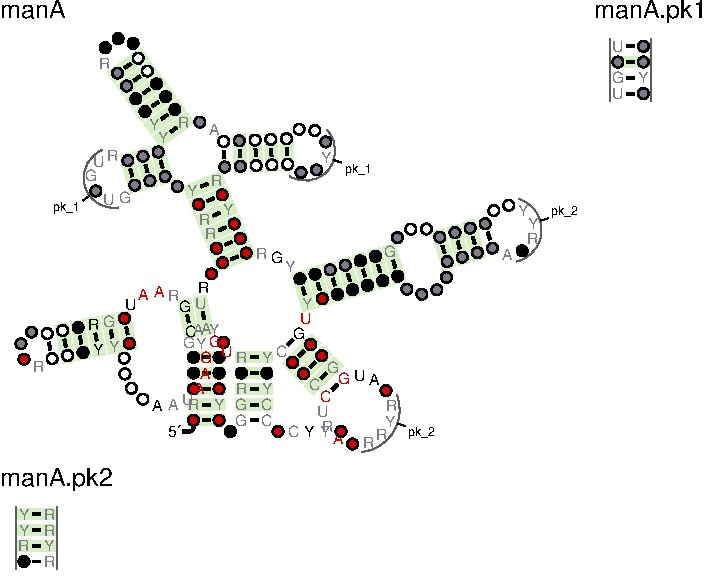
\includegraphics[scale=0.7]{manA_R2R.pdf} 
  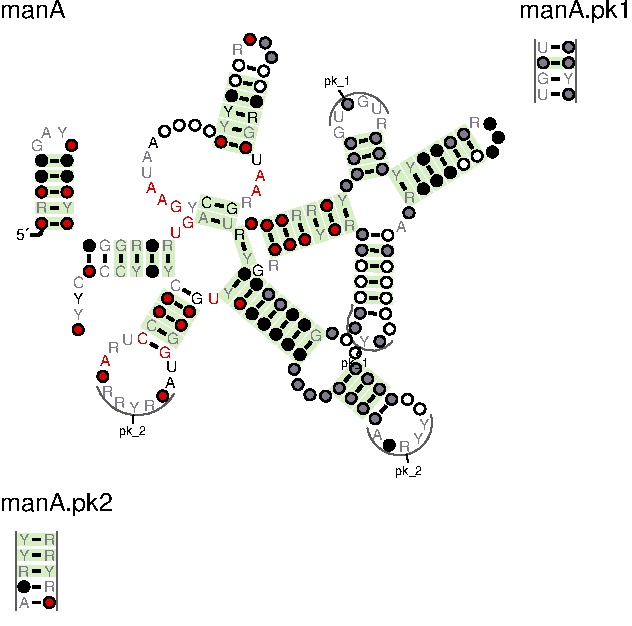
\includegraphics[scale=0.7]{manA_fold_R2R.pdf} 
  \caption{\small\textbf{Left:}
    \emprog{tutorial/manA.R2R.sto.\{pdf,svg\}}, the consensus
    secondary structure given in the input alignment, depicted by
    \rscape, using the program R2R.  \textbf{Right:}
    \emprog{tutorial/manA.fold.R2R.sto.\{pdf,svg\}}, The consensus
    structure produced by \rscape\ (option --cacofold).  Base pairs with
    covariation scores equal or below the target E-value (0.05 as
    default) are depicted in green.  }
 \label{fig:manA_r2r}
 \end{figure}
 

 \subsection{Single sequence structure prediction}

 If the alignment includes only one sequence, no statistical test is performed. \\

 \noindent
 \user{bin/R-scape --cacofold tutorial/manA-oneseq.sto}\\
%
 reports the best structure given the sequence. No covariation support
 is possible for any of the basepairs reported from this
 analysis. Structures produced this way have to taken with great
 skepticism. 

 \subsection{Default parameters}

Default parameters are:

\begin{sreitems}{\emprog{Pairwise percent identity:}}
\item[\emprog{Target E-value:}]default is 0.05. \rscape\, reports
  pairs which covariation score has E-value smaller or equal to the
  target value.  The target E-value can be changed with option
  \emprog{-E <x>}, $x >= 0$.

\item[\emprog{Sequence weighting:}]Sequences are weighted according to
  the Gerstein/Sonnhammer/Chothia (GSC)
  algorithm~\citep{Gerstein94}. This algorithm is time consuming. For
  alignments with more than 1000 sequences, we use the faster
  position-based weighting algorithm~\citep{Henikoff94b}. Both
  weighting algorithms are implemented as part of the easel library.

\item[\emprog{Gaps in columns:}]Columns with more than 50\% gaps are
  removed. The gap threshold for removing columns can be modified
   using option \emprog{--gapthresh <x>} , $0<x<=1$.

 \item[\emprog{Covariation statistic:}]The default covariation statistic
   is the average product corrected G-Test (equivalent to option
   \emprog{--GTp}).

 \item[\emprog{Covariation Class:}]\rscape\ uses the 16 component
   covariation statistic (C16), unless the number of sequences in the
   alignment is $\leq$ 8 or the length of the alignment is $\leq$ 50,
   in which case it uses the two-class covariation statistic (C2). A
   particular covariation class can be selected using either
   \emprog{--C16} or \emprog{--C2}.

   The threshold for the minimum number of sequences can be changed
   with option \prog{--nseqthresh <n>}.  The threshold for the minimum
   alignment length can be changed with option \prog{--alenthresh <n>}.

 \item[\emprog{Null alignments:}]In order to estimate E-values,
   \rscape\ produces 20 null alignments, unless the product of the
   number of sequences by the length of the alignment $<$ 10,000 in
   which case the number of null alignments is 50; or $<$ 1,000 in
   which case it is 100. The number of null alignments can be
   controlled with option \emprog{--nshuffle <n>}.
 \end{sreitems}

 A full list of the \rscape\ options is found by using

 \user{\rscape\ -h}

 
 


\newpage
\input{input}

\newpage
\label{section:outputs}
\setcounter{footnote}{0}
\section{Outputs}

For each alignment file \prog{rnafile.sto}, \rscape\, produces the
following output files:

\begin{sreitems}{\emprog{rnafile.sorted.out}}
\item[\emprog{rnafile.out}] Tabular output with the significant pairs,
  with their score and E-value.
%
\item[\emprog{rnafile.sorted.out}] Tabular output sorted from highest to
  lowest E-value.
%
%
\item[\emprog{rnafile.sum}] Tabular output with a line summary statistics
  per alignment in the file.
%
\end{sreitems}

\subsection{Tabular output per input file}

The distribution includes in the directory tuturials/ examples of
output files. If you run \rscape, the outputs will go into your
current working directory (not necessarily tutorials/).

The output file \emprog{tutorial/updated\_Arisong.out} looks like this:
\user{more tutorial/updated\_Arisong.out}

\begin{sreoutput}
# MSA updated_Arisong_1 nseq 95 (95) alen 65 (150) avgid 66.35 (64.97) nbpairs 20 (20)
# GammaFIT: pmass 0.050024 mu 19.840474 lambda 0.152973 tau 1.281689
# Method Target_E-val [cov_min,conv_max] [FP | TP True Found | Sen PPV F] 
# GTp    0.05           [-9.64,121.98]    [0 | 11 20 11 | 55.00 100.00 70.97] 
#       left_pos       right_pos        score   E-value
#------------------------------------------------------------
*               94             110      56.89   0.00598452
*               96             108      89.19   4.97828e-05
*               97             107      52.27   0.0117527
...
\end{sreoutput}
The output file is a tabular list of significant pairs sorted by sequence positions:

\begin{sreitems}{\prog{Second and third columns}}
 \item[\prog{First column}] indicates whether the significant pair is
   part of the given structure (*), or not.  If the pair is not in the
   structure, we distinguish whether the pair is compatible with the
   given structure ($\sim$) or not (blank).

  In addition, if the structure is provided by a PDB file (using the
  option \prog{--pdbfile}), a non Watson-Crick/Watson-Crick base pair
  is designated by ``**''. A contact that is not a basepair is
  designated by: ``$c\sim$'' if compatible with all the basepairs, or
  by ``$c$'' otherwise.

 \item[\prog{Second and third columns}] are the two positions of the
   pair, $i\leq j$ respectively. Positions are relative to the input
   alignment.

 \item[\prog{Fourth column}] is the covariation score.

 \item[\prog{Fifth column}] is the E-value. Significant positions
   have E-values $<< 1$.
 \end{sreitems}
 The output file also includes two comment lines per alignment in the
 file:

 \begin{sreitems}{\prog{Second comment line}} \item[\prog{First
 comment line}]describes properties of the alignment: number of
 sequence (nseq), alignment length (alen), average percentage identity
 (avgid), and number of base pairs (nbpairs).  Values in parentheses
 correspond to the alignment as given. Values not in parentheses
 correspond to the analyzed alignment after the filters (for redundant
 sequences and gapped columns) have been applied.

 \item[\prog{Second comment line}]describes properties of the \rscape\
   search: the covariation method (GTp), the E-value threshold (0.05),
   the range of scores for all pairs in the alignments (from -9.7 to
   89.1), the number of covarying non base pairs (0), the number of
   covarying base pairs (11), the number of base pairs (20), and the
   total number of covarying pairs (11). Lastly we provide the
   sensitivity (SEN=55.00=11/20), positive predictive value
   (PPV=100.00=11/11), and F-measure (F=70.97 = 2 * SEN * PPV /
   (SEN+PPV)).  \end{sreitems}


\subsection{Other tabular outputs}

 \rscape\ produces two more tabular outputs per input file that are
 more relevant for benchmarking purposes, those are:\\

 File \emprog{tutorial/updated\_Arisong.sum} looks like:

\user{more tutorial/updated\_Arisong.sum}
 \begin{sreoutput}
 #target_E-val   MSA                     nseq    alen    avgid    method  TP      True    Found   SEN     PPV
 0.05            updated_Arisong_1       95      65      66.35    GTp     11      20      11      55.00 100.00 
\end{sreoutput}
 This file produces a one line output per alignment in the file.
 \begin{sreitems}{\prog{Second column}}
 \item[\prog{Column 1}] Target E-value.
 \item[\prog{Column 2}] Alignment name.
 \item[\prog{Column 3}] Number of sequence in the analyzed alignment.
 \item[\prog{Column 4}] Number of columns analyzed.
 \item[\prog{Column 5}] Average percentage identity in the analyzed alignment.
 \item[\prog{Column 6}] Covariation statistic.
 \item[\prog{Column 7}] Number of significant base pairs, TP  (true positives).
 \item[\prog{Column 8}] Number of base pairs, T (True).
 \item[\prog{Column 9}] Number of significant pairs, F (Found).
 \item[\prog{Column 10}] Sensitivity = TP/T.
 \item[\prog{Column 11}] Positive predictive value = TP/F.

 \end{sreitems}

\subsection{Outputs per alignment}

A Stockholm alignment file can include several different multiple
sequence alignments (MSAs).  \rscape\ produces the following output
files, one for each individual alignment in the input Stockholm file:

\subsubsection{Alignment with consensus secondary structure}
If the given alignment  has a consensus secondary structure
(\prog{\#=GF SS\_cons} markup), the following files are produced

\begin{sreitems}{\emprog{rnafile\_msaname.R2R.sto.\{pdf,svg\}}}
\item[\emprog{rnafile\_msaname.R2R.sto}] Stockholm file annotated by a
  modified version of the R2R program. This file includes the
  information necessary to draw the consensus structure, and to
  annotate the significantly covarying base pairs.
%
\item[\emprog{rnafile\_msaname.R2R.sto.\{pdf,svg\}}] Drawing of the
  \rscape-annotated consensus secondary structure.
%
\item[\emprog{rnafile\_msaname.surv}] A two column file with the 
survival functions (surv) for the covariation scores.
%
\item[\emprog{rnafile\_msaname.surv.ps}] Plot of the score's survival function
$P(X > \mbox{score})$. Drawing this
file requires that program \emprog{gnuplot} is installed somewhere in
the
\prog{\$\{PATH\}}, or that the environmental variable GNUPLOT 
pointing to a gnuplot executable is defined.
%
\item[\emprog{rnafile\_msaname.dplot.\{ps,svg\}}] Dot plot of the consensus
  secondary structure annotated according to covariation. Drawing of this
file requires that program \emprog{gnuplot} is installed somewhere in the
\prog{\$\{PATH\}}, or that the environmental variable GNUPLOT 
pointing to a gnuplot executable is defined.
%
\end{sreitems}
For each alignment, \emprog{msaname} is given
by \prog{<ACC>\_<ID>}, the combination of the accession \prog{\#=GF
AC <ACC>} and name \prog{\#=GF ID <ID>} in the Stockholm-format markups (or
one of two if the other in not defined).  If none of those fields are
defined, \emprog{msaname} is a number describing the order in the
file of the given alignment.

\subsubsection{Alignment without consensus secondary structure}
Alternatively, if the alignment does not have a consensus secondary
structure (or if it does and the option \prog{\rscape\ --cyk} is
used) \rscape\, produces the following files describing the
maximal-covariation optimal secondary structure:

\begin{sreitems}{\emprog{rnafile\_msaname.cyk.R2R.sto.\{pdf,svg\}}}
\item[\emprog{rnafile\_msaname.cyk.R2R.sto}]
%
\item[\emprog{rnafile\_msaname.cyk.R2R.sto.\{pdf,svg\}}]
%
\item[\emprog{rnafile\_msaname.cyk.surv}]
%
\item[\emprog{rnafile\_msaname.cyk.surv.\{ps.svg\}}]
%
\item[\emprog{rnafile\_msaname.cyk.dplot.\{ps,svg\}}]
%
\end{sreitems}
These files are formatted identically to those for describing the given
consensus structure.


\subsubsection{Details about outputs per alignment}
 Two files are produced per alignment in the input file: \\

 File \emprog{tutorial/updated\_Arisong\_1.R2R.sto} is a Stockholm
 formatted alignment that includes the input alignment annotated with
 the consensus structure. This Stockholm file also includes the
 additional annotation required to use the drawing program R2R.

 It is possible that the resulting drawing will show parts of the
 secondary structure occluded from each other (especially for long
 RNAs).  Using this file, one can customize a different drawing of the
 structure using the R2R documentation, provided in
 \prog{lib/R2R/R2R-manual.pdf}.\\

 File \emprog{tutorial/updated\_Arisong\_1.surv} looks like this:

\user{more tutorial/updated\_Arisong.surv}
 \begin{sreoutput}
121.795428      0.05
95.862635       0.1
89.113004       0.15
...
 &
63.890698       0.000485437
58.917286       0.000970874
47.904730       0.00145631
...
 &
81.652885       2.40385e-06
77.745204       4.80769e-06
77.034717       7.21154e-06
...
 &
256.788050      2.64342e-17
256.432807      2.7899e-17
256.077563      2.94449e-17
...
 &
 \end{sreoutput}
 The first column is a covariation score (x). The second column is the
 survival function $P(X > x)$, that is the frequency of pairs having
 score larger than x. The file includes four survival functions separated by a
 ``\&'' line. The three survival functions correspond to:

 \begin{sreitems}{\prog{Second function:}}
 \item[\prog{First functions:}] the given alignment, proposed base pairs.
 (This section is empty if no secondary structure is proposed.)
 \item[\prog{Second functions:}] the given alignment, not proposed pairs.
 \item[\prog{Third function:}] the aggregation of all null alignments, all possible pairs.
 \item[\prog{Fourth function:}] the expected null survival function according to the tail Gamma fit.
 \end{sreitems}


\clearpage
\subsubsection{Graphical outputs per alignment}
 Three plots are produced per alignment in the input file: 

 \begin{figure}[h]
   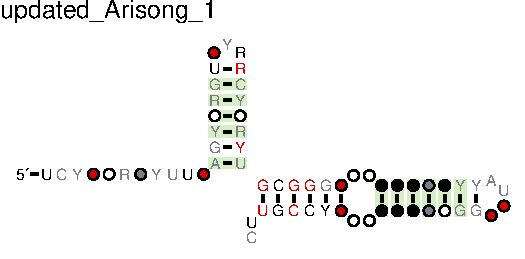
\includegraphics[scale=1.5]{Arisong_R2R.pdf} 
 \caption{\small\textbf{\emprog{tutorial/updated\_Arisong\_1.R2R.sto.\{pdf,svg\}}:
     annotated consensus secondary structure.} Base pairs with
   covariation scores equal or below the target E-value (0.05 as
   default) are depicted in green. By default only positions in the
   alignment with more than 50\% occupancy are depicted (unless they form
   a base pair). Option \prog{--r2rall} forces the depiction of all
   positions in the alignment.  }
 \label{fig:r2r}
 \end{figure}

 \begin{figure}[h] 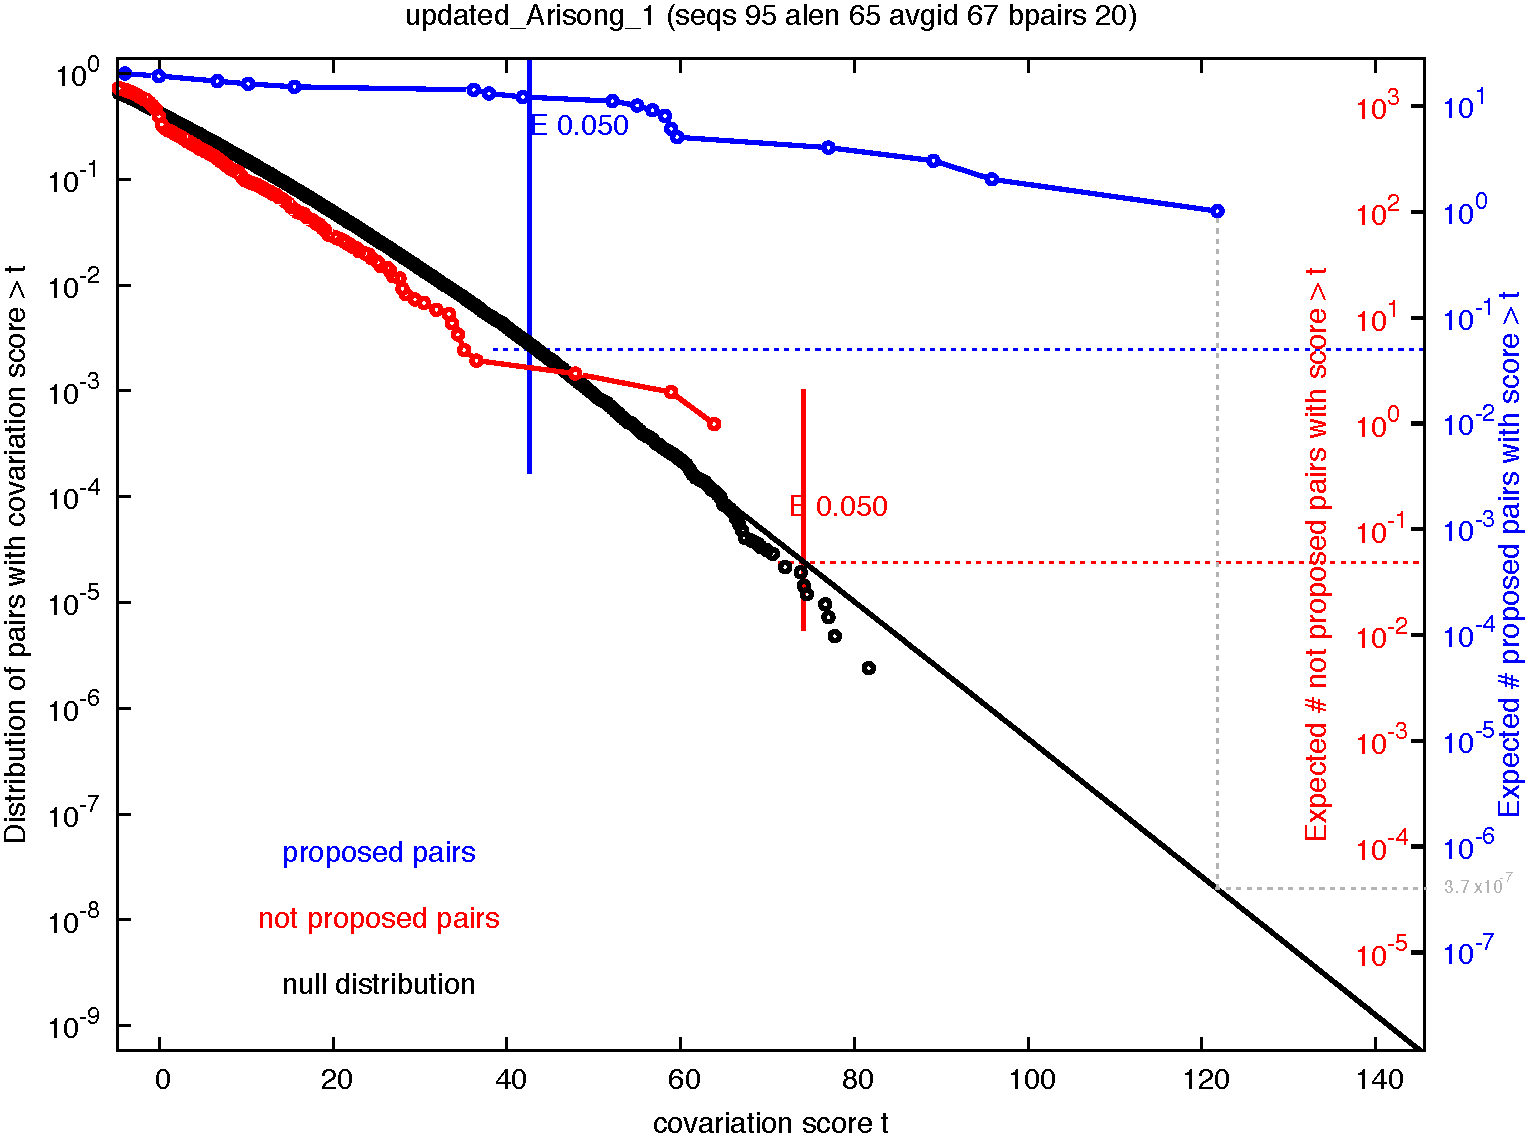
\includegraphics[scale=0.50]{Arisong_surv.pdf}
 \caption{\small\textbf{\emprog{tutorial/updated\_Arisong\_1.surv.\{ps,svg\}}:
 covariation scores survival function $P(X>x)$.}  The survival
 function of scores for all pairs in the given alignment is depicted
 in blue. The survival function for the null alignments is depicted in
 black. A black line indicates to fit to a truncated Gamma
 distribution of the tail of the null distribution. In red, we plot
 the survival function of scores for the pairs in the given alignment
 excluding those proposed as base pairs. For a particular pair, as an
 example the highest scoring one from the distribution of proposed
 pairs (blue), we obtain its E-value by drawing a vertical (gray) line
 from the point to the null distribution (black). The corresponding
 value in the blue scale gives us the E-value for that pair (in this
 example, 3.7 $\cdot$10$^{-7}$).
 }
 \label{fig:surv}
 \end{figure}

 \begin{figure}[h] 
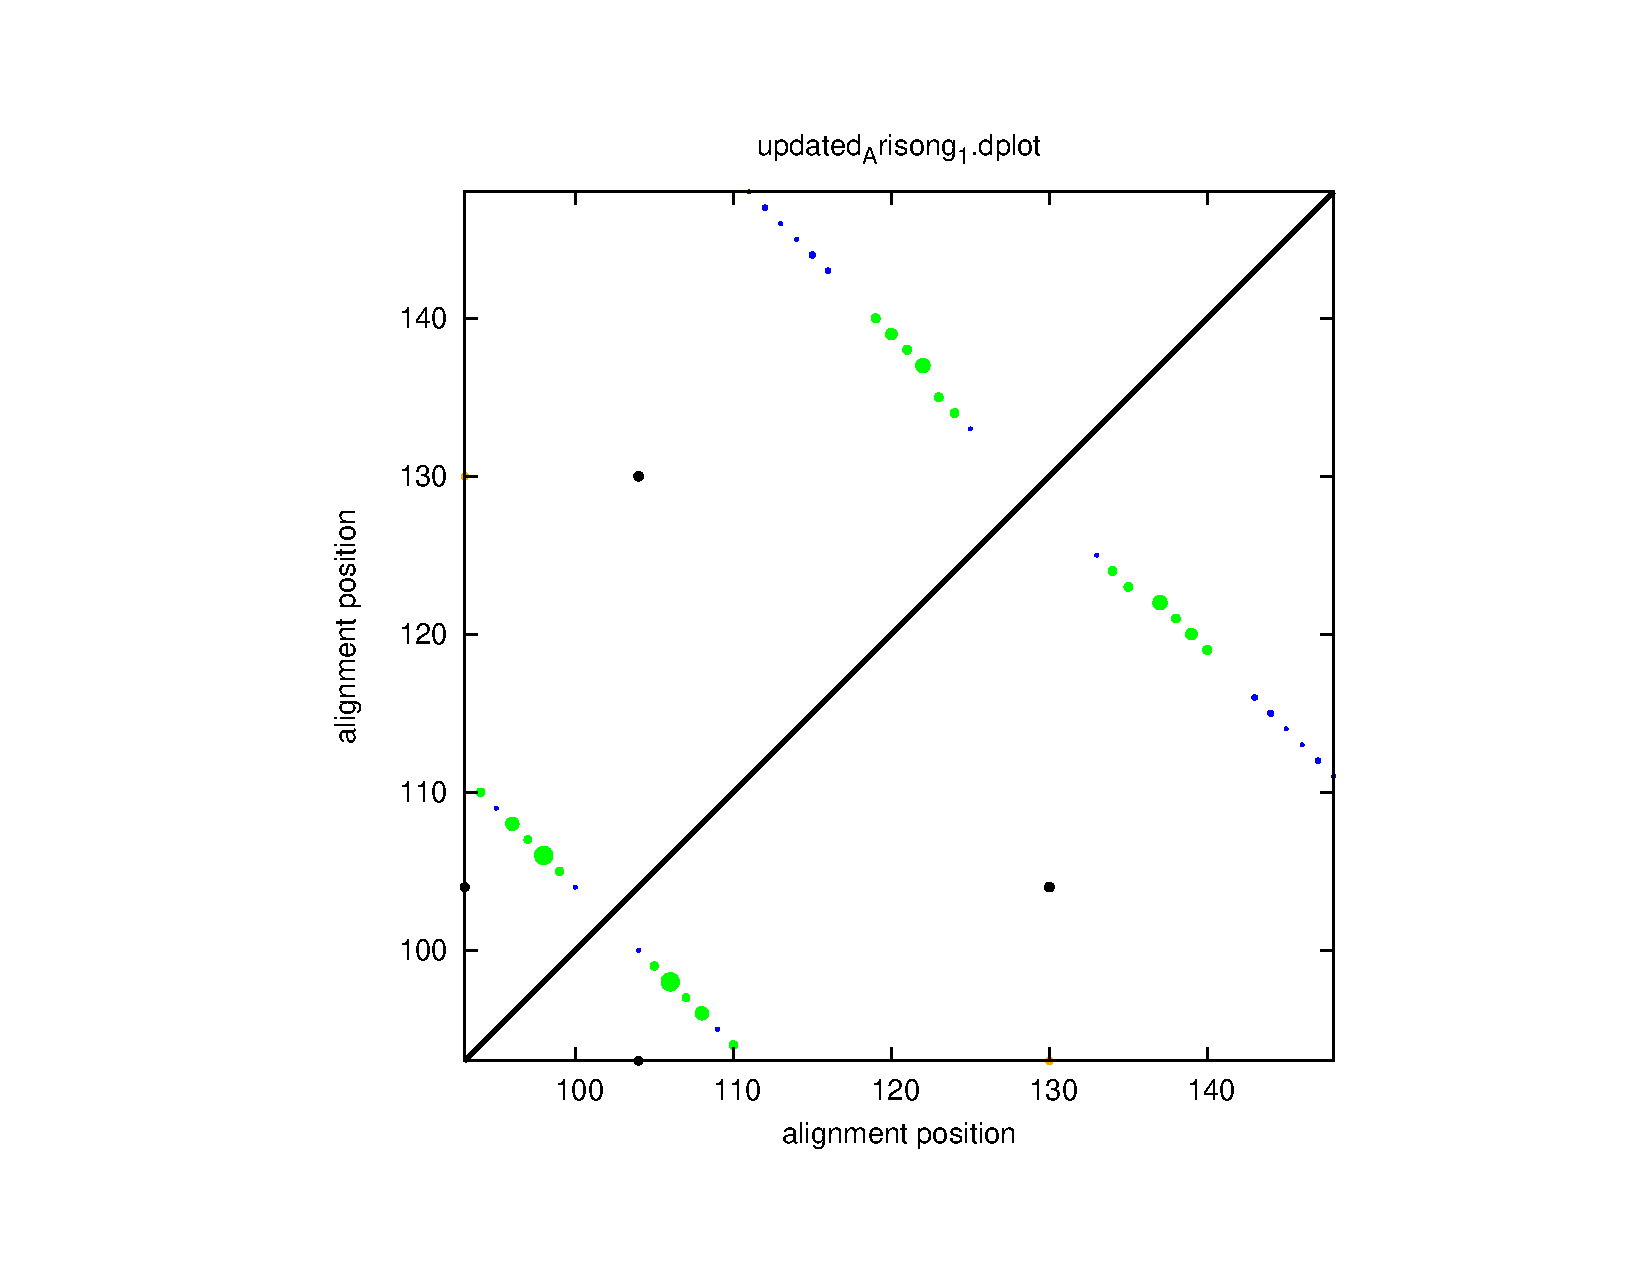
\includegraphics[scale=0.60]{Arisong_dplot.pdf} 
 \caption{\small\textbf{\emprog{tutorial/updated\_Arisong\_1.dplot.\{ps,svg\}}:
   dotplot.}  Dot size is proportional to the covariation score. In
   blue we depict the consensus base pairs; in green, the consensus
   base pairs that show significant covariation; in orange (none shown
   in this plot), we depict other pairs that have significant
   covariation, are not part of the consensus secondary structure but
   are compatible with it; in black we depict other significant pairs.
   Position are relative to the original input alignment (before any
   gapped column is removed).}
\label{fig:dplot} 
\end{figure}



 



\newpage
\clearpage
\section{Options}
\label{section:options}
\setcounter{footnote}{0}

The whole list of options can be found using 

\user{R-scape -h}\\

Some important options are:
\subsection{Covariation statistic options}

\subsubsection{\prog{-E <x>}}  Target E-value is $x\geq 0$.

\subsubsection{\prog{--GT, --MI,  --MIr, --MIg, --CHI, --OMES, --RAF, --RAFS, }}
We favor the G-test covariation statistic, but a total of eight
covariation statistics are currently implemented in \rscape. For each
covariation statistic (GT, for instance), \rscape\ can also calculate
its average product correction (GTp) and its average sum corrections
(GTa). For each option above, appending ``p'' or ``a'' chooses one of the
corrections. For example, \prog{--GT} does the G-test statistic,
\prog{--GTp} does the APC-corrected G-test statistic, \prog{--GTa}
does the ASC-corrected G-test statistic.\\

The \rscape\ default is \prog{--GTp}.\\

Details of the definition and provenance of the different covariation
statistics can be found in the \rscape\ manuscript: Rivas, E. \& Eddy
S.~E., \textit{``A statistical test for conserved RNA structure shows
lack of evidence for structure in lncRNAs''}.

\noindent
In a nutshell, given two
alignment columns $i,j$,
%
\[
\begin{array}{lrcl}
  \mbox{G-test:\citep{Woolf1957}}                                       & \mathrm{GT}(i,j)   & = & 2 \, \sum_{a,b} \mathrm{Obs}^{ab}_{ij} \, \log \frac{ \mathrm{Obs}^{ab}_{ij} } { \mathrm{Exp}^{ab}_{ij} }, \\
  \mbox{Pearson's chi-square:}                                          & \mathrm{CHI}(i,j)  & = &      \sum_{a,b} \frac{ \left(\mathrm{Obs}^{ab}_{ij} - \mathrm{Exp}^{ab}_{ij}\right)^2 }{\mathrm{Exp}^{ab}_{ij}},\\ 
  \mbox{Mutual information:\citep{Shannon48,Gutell94b}}                 & \mathrm{MI}(i,j)   & = &      \sum_{a,b} P^{ab}_{ij} \, \log \frac{ P^{ab}_{ij} }{ p^{a}_{i} \, p^{b}_{j}},                       \\
  \mbox{MI normalized:\citep{Martin05}}                                 & \mathrm{MIr}(i,j)  & = & \frac{\mathrm{MI}(i,j)} {H(i,j)} = \frac{\mathrm{MI}(i,j)} { -\sum_{a,b} P^{ab}_{ij} \log  P^{ab}_{ij}},        \\
  \mbox{MI with gap penalty:\citep{LindgreenKrogh06}}                   & \mathrm{MIg}(i,j)  & = & \mathrm{MI}(i,j) - \frac{N^G_{ij}} {N},                                                                   \\
  \mbox{Obs-Minus-Exp-Squared:\citep{Fodor04}}                          & \mathrm{OMES}(i,j) & = &      \sum_{a,b} \frac{ \left(\mathrm{Obs}^{ab}_{ij} - \mathrm{Exp}^{ab}_{ij}\right)^2 }{N_{ij}},                \\
  \mbox{RNAalifold (RAF):\citep{Hofacker02}}                            & \mathrm{RAF}(i,j)  & = & \mathrm{B}_{i,j},                                      \\
  \mbox{RNAalifold Stacking (RAFS):\citep{LindgreenKrogh06}}            & \mathrm{RAFS}(i,j) & = & \frac{1}{4}\left(\mathrm{B}_{i-1,j+1}+2\,\mathrm{B}_{i,j}+\mathrm{B}_{i+1,j-1}\right).                                      \\
\end{array}
\]
%
\noindent
where $a,b$ are (non-gap) residues; $N$ is the total number of aligned
sequences; $\mathrm{Obs}^{ab}_{ij}$ is the observed count of $a:b$
pairs in columns $i,j$ (only counting when both a,b are residues);
$N_{ij}$ is the total number of residue pairs in columns $i,j$ (only
counting when both a,b are residues); $P^{ab}_{ij}$ is the observed
frequency of pair $a:b$ in columns $i,j$
($P^{ab}_{ij}=\frac{Obs^{ab}_{ij}}{N_{ij}}$); $\mathrm{Exp}^{ab}_{ij}=
N_{ij} p^a_ip^b_j$ is the expected frequency of pair $a:b$ assuming
$i,j$ are independent, where $p^a_i$ are the marginal frequencies of
$a$ residues in column $i$ (averaged to all other positions) ($p^a_i
= \frac{1}{L-1}\sum_{j\neq i} \sum_b P^{ab}_{ij}$); $N^G_{ij} = N -
N_{ij}$ is the number of pairs involving at least one gap symbol; the
definition of $\mathrm{B}_{i,j}$ used in the RAF and RAFS statistics
is involved, a concise definition can be found
elsewhere~\citep{LindgreenKrogh06}.

The background corrections~\citep{DunnGloor07} for a given
covariation statistic above $\mathrm{COV}(i,j)$ are,
%
\[
\begin{array}{lrcl}
  \mbox{\small Average product correction} & \mathrm{COVp}(i,j) & = &  \mathrm{COV}(i,j) - \frac { \mathrm{COV}(i) \mathrm{COV}(j) } { \mathrm{COV} }, \\
  \mbox{\small Average sum correction}     & \mathrm{COVa}(i,j) & = &  \mathrm{COV}(i,j) - \left( \mathrm{COV}(i) + \mathrm{COV}(j) - \mathrm{COV} \right). \\
\end{array}
\]



\subsubsection{\prog{--C2, --C16}}
For all the covariation statistics (except RAF and RAFS), one can do a
16-component (C16) or a two-component (C2) calculation, depending on
whether it uses the 16 possible pair combinations, or those are group
in two classes depending on whether they form a Watson-Crick pair (6
cases, including U:G and G:U), or whether they do not (10 cases).

\rscape's default is the 16 component covariation statistic, unless
the number of sequences in the alignment is $\leq$ 8 or the length of
the alignment is $\leq$ 50, in which case it uses the two-class
covariation statistic.

\subsection{Search options}


\subsubsection{\prog{-s}} The ``two-set test'' option.
This option requires that a structure is provided with the alignment.
If option \prog{-s} is used, \rscape\ performs two independent test,
one for the given structure, another for all other possible pairs.
The default is a ``one-set test'' in which all possible pairs in the
alignment are tested equivalently.


\subsubsection{\prog{--fold}} A CaCoFold structure is computed that includes all significant base pairs. All files related to this 
CaCoFold structure include the suffix \prog{.fold.}

When option \prog{--fold} is used, a file with the original alignment  annotated with the R-scape structure in Stockholm format is produced.
This alignment has the suffix \prog{.fold.sto}.

\subsubsection{\prog{--naive}} Reports the laundry list of all covariation scores, without any statistical significance (E-value)
associated to them. No null alignments are created.

\subsubsection{\prog{--tstart <n>}} Analyze starting from position $n >= 1$ in the alignment.

\subsubsection{\prog{--tend <n>}} Analyze ending at position $n <= L$ in the alignment.

\subsubsection{\prog{--window <n>}} \rscape\ can be run in a window scanning version for long alignments.
The window size is $n>0$.

\subsubsection{\prog{--slide <n>}} In scanning mode, this options sets the number of positions to move from window to window, $n >0$.

\subsubsection{\prog{--vshuffle}} Vertical shuffle, a developers tool. Before performing any analysis, it shuffles all residues in each alignment column independently.

\subsubsection{\prog{--cshuffle}} Column shuffle, a developers tool. Before performing any analysis, it shuffles all columns in the alignment.

\subsubsection{\prog{--givennull <f>}} Use histrogram provided in file $<f>$ as null. 



\subsection{Input alignment options}

\subsubsection{\prog{-I <x>}} Only sequences with less than $0<x\leq 1$
pairwise similarity are considered in the analysis.  Pairwise \%
identity is defined as the ratio of identical positions divided by the
minimum length of the two sequences. If this option is not used all
(weighted) sequences are used in the analysis.

\subsubsection{\prog{--gapthresh <x>}} Only columns with less than $0<x\leq 1$ fraction of gaps are considered in the analysis.

\subsubsection{\prog{--consensus}} If the alignment has a GC ``seq\_cons'' field, only consensus positions will be analyzed.

\subsubsection{\prog{--submsa <n>}} Analyzes a random subset of the input alignment.

\subsubsection{\prog{--treefile <f>}} A phylogenetic tree in Newick format can be given (by default a tree is created 
from the alignment using the program FastTree~\citep{Price10}).  \rscape\ checks that the  number of taxa and the names
of the taxa matches for all alignments analyzed.


\subsection{Options for producing a CaCoFold structure}

\subsubsection{\prog{--fold}}  
When using the option \prog{--fold}, R-scape engages the CaCoFold
algorithm to produce a predicted structure. The CaCoFold algorithm
incorporates all positive (significantly covarying) basepairs, and
prevents any negative pair (pairs that have power of covariation but
not covariation) from happening. The CaCoFold algorithm uses a
recursive cascade of constrained foldings. The first fold uses the RBG probabilistic grammar, the rest use the G6X probabilistic grammar.

\noindent
Regarding the predicted structure, CaCoFold can use one two algorithms:

\subsubsection{\prog{--cyk}}        Default option. Each folding reports the structure with the best probability using the CYK algorithm.

\subsubsection{\prog{--decoding}}   This options returns the structure obtained by posterior decoding.

\noindent
Posterior decoding usually performs better than CYK. Both algorithm has the same algorithmic complexity. CYK is faster.

\noindent
Several additional options can be used in combination with   \prog{--fold},

\subsubsection{\prog{--refseq}}   By default the CaCoFold algorithm folds a profile sequence built from the alignment. Using this option, the sequence to fold is a consensus reference sequence.

\subsubsection{\prog{--E\_neg <x>}}   Pairs with E-value larger than the E-value cutoff but smaller than <x> will not be called negatives regardless of their covariation power. Default for E\_neg is 1.0.

\subsubsection{\prog{--lastfold}} This option forces one last alternative fold (using grammar G6X) after all covarying basepairs have already been
integrated into the structure. By default this last fold is not
performed. In the absence of any covarying basepair, one fold is
performed using grammar RBG.

\subsubsection{\prog{--show\_hoverlap}} This option leaves the alternative helices unmodified. By default, alternative structures are trimmed down to show no overlap with helices from the previous layers.

\subsubsection{\prog{--covmin <n>}} Minimum distance between position to report significant covariations. Default is 1, which means that significant covariations between
contiguous positions are reported.

\subsubsection{\prog{--allow\_negatives}} This option (just for developers) allows all basepairs to form regardless of their power.

\subsection{Options for importing a structure}

\rscape\ does not require to input a structure (either a RNA structure
or a protein contact map). By default \rscape\ analyzes all possible
pairs in the alignment.
\vspace{1mm}

\noindent
There are two ways to provide a contact map (or structure):

\begin{itemize}

\item By providing the alignment in Stockholm format with a ``ss\_cons'' field including the consensus
structure for the alignment. (For RNA alignments only.)

\item By analyzing a 3D structure provided in a PDB file. (For either RNA or peptide alignments.)\\
\end{itemize}

\noindent
These two methods can be combined together. For a nucleotide
alignment, if both a consensus structure is present in the alignment,
and a PDB file is provided (using option \prog{--pdb}), the
consensus structure will be extended by the information provided by
the pdbfile.  To ignore the consensus structure use
option \prog{--onlypdb}.\\


\noindent
From the PDB file we obtain three types of structural pairs:

\begin{itemize}
\item \textbf{Contacts:} defined as those two residues at a close spatial distance (specified by the user with option \prog{--cntmaxD}).
\item \textbf{Basepair:} RNA basepairs. \\
RNA basepairs are calculated using the program \prog{rnaview}~\citep{YangWesthof03}.

These RNA basepairs can be further classified in two types:
\begin{itemize}
\item \textbf{Watson-Crick basepairs:} the canonical RNA basepairs. mostly A:U, G:C, or G:U pairs. (H-bond interactions between two W-C faces in cis).
\item \textbf{Other basepairs:} the non-canonical RNA basepairs (all other types of H-bond interactions, 12 different types).
\end{itemize}
\end{itemize}

Contacts and RNA basepairs are extracted as follows:
\begin{itemize}

\item The spatial distance between any two residues is calculated as the  minimal Euclidean distance between any two atoms (excluding
 H atoms). Any two pairs at a distance not larger than a maximum value
(\texttt{contmaxD}) are called a ``contact''.

\item RNA basepairs are obtained using the program \texttt{rnaview}~\citep{YangWesthof03}\\
(http://ndbserver.rutgers.edu/ndbmodule/services/download/rnaview.html).\\
The RNA basepair annotation takes precedent over the annotation as ``contact''.
\end{itemize}

\vspace{2mm}
\noindent
The options that control the input of a structure or contact map are:

\subsubsection{\prog{--pdb <s>}} Reads a pdbfile associated to the alignment, and extracts the contacts
from it.

A ``.cmap'' file is produced reporting the structure obtained from the PDB file.

Option \prog{--pdb} is incompatible with \prog{--fold}.

\subsubsection{\prog{--cntmaxD <x>}} Maximum distance (in Angstroms) allowed between two residues to define a ``contact'' is $\langle x\rangle$.

\subsubsection{\prog{--cntmind <n>}} Minimum distance (in residue positions) in the backbone between two residues required to define a ``contact'' is $\langle n\rangle$.
\vspace{5mm}

\subsubsection{\prog{--onlypdb}} Reads the structure from the pdbfile and ignores the alignment consensus structure (if provided).

\subsubsection{\prog{--draw\_nonWC}} Adds the non-canonical basepairs into the structure graphical output. For clarity, the default is to draw only the Watson-Crick basepairs.
This option affects only the drawing of the structure. All basepairs (canonical or not) are used as part of the structure to perform the two-set statistical test.
\\\\

\noindent
Example of reading a structure from a PDB file for the FMN riboswitch:

\user{bin/R-scape --cntmaxD 4 --cntmind 3 --pdb tutorial/3f2q.pdb -s --onlypdb tutorial/RF00050.sto}\\

\noindent
This command line extracts contacts from the pdb file that are at a
Euclidean distance $\leq 4 \AA$ in the PDB structure, and such that
they are at least 3 residues apart in the backbone.


\noindent
The output is

\begin{sreoutput}
# R-scape :: RNA Structural Covariation Above Phylogenetic Expectation
# R-scape 0.8.1 (Jul 2018)
# Copyright (C) 2016 Howard Hughes Medical Institute.
# Freely distributed under the GNU General Public License (GPLv3).
# - - - - - - - - - - - - - - - - - - - - - - - - - - - - - - - - - - - -
# Two-set statistical test (one test for annotated basepairs, another for all other pairs)
#
# Structure obtained from the pdbfile
# ij in alignment | ij in pdbsequence | basepair type
# 3 218 | 1 112 | WWc
# 4 216 | 2 110 | CONTACT
# 4 217 | 2 111 | WWc
# 4 218 | 2 112 | CONTACT
# 5 216 | 3 110 | WWc
# 5 217 | 3 111 | CONTACT
# 6 215 | 4 109 | WWc
# 6 216 | 4 110 | CONTACT
# .
# .
# .
# 192 202 | 87 96 | WWc
# 192 203 | 87 97 | CONTACT
# 193 198 | 88 92 | CONTACT
# 193 201 | 88 95 | WWc
# 193 202 | 88 96 | CONTACT
# 195 197 | 89 91 | CONTACT
# 195 198 | 89 92 | WHt
# 198 200 | 92 94 | CONTACT
# 198 201 | 92 95 | CONTACT
# 205 207 | 99 101 | CONTACT
# PDB:      versions/rscape/rscape_v0.8/tutorial/3f2q.pdb
# contacts  169 (49 bpairs 35 wc bpairs)
# maxD      4.00
# mind      3
# distance  MIN
# L         139
# alen      221
# pdblen    112
# ::[[[[[[[[,,,,,,<<<_______>>>,((((<<<<_________________AA>>>>,,<<<----------<____>>>>,,,<<<<<_______>>>>>aa))AAAA----))aaaa,,,,,,]]]]]]]]::
# MSA RF00050_FMN.3f2q nseq 144 (144) alen 139 (221) avgid 69.18 (68.15) nbpairs 49 (0)
#
# Method Target_E-val [cov_min,conv_max] [FP | TP True Found | Sen PPV F] 
# GTp    0.05         [-9.78,216.11]     [1 | 14 49 15 | 28.57 93.33 43.75] 
#
#       left_pos       right_pos        score           E-value
#------------------------------------------------------------------
*	     171	     183	216.11095	1.6421e-10
*	     170	     184	211.69081	2.76699e-10
*	     192	     202	168.72417	4.95548e-08
*	       8	     213	149.71776	4.89982e-07
*	     172	     182	138.66664	1.84675e-06
*	     169	     185	137.23189	2.21548e-06
**	      16	      30	133.44999	3.53772e-06
*	       5	     216	131.02575	4.70876e-06
*	      84	     186	125.60806	9.0169e-06
*	      17	      29	112.04610	4.62895e-05
*	       7	     214	111.12654	5.13519e-05
*	       6	     215	96.43781	0.00029929
*	      36	      87	96.32752	0.00029929
*	      94	     163	78.81578	0.0024303
 	       7	     213	107.68588	0.0147937
\end{sreoutput}

\noindent
All coordinates are relative to the input alignment. The annotation of
all types of RNA basepairs (WWc, WWt, WHc,...) is produced by the
program \prog{rnaview}~\citep{YangWesthof03}.

\subsection{Options for type of pairs tested}

When performing the two-class statistical test (option \prog{-s})
using a pdbfile to read the structure, there are different options as
to which types of basepairs are used to define the sample size for the
basepairs test.

The options are:

\subsubsection{\prog{--samplecontacts}}
The basepair statistical test includes all the contacts identified in a PDB
or/and as a RNA secondary structure included with a input alignment in
Stockholm format.  This is the default option for amino acid
alignments if a PDB file is provided.  

\subsubsection{\prog{--samplebp}} For RNA alignments with only.
The basepair statistical test includes basepairs of all 12 possible types.
This is the default option for RNA/DNA alignments if a PDB file is
provided.  

\subsubsection{\prog{--samplewc}} For RNA alignments only.
The basepair statistical test includes only the canonical
(Watson-Crick/Watson-Crick type) basepairs (A:U, G:C, G:U).  This is
the default option for RNA/DNA alignments if a consensus secondary
structure is provided. 

\subsection{Output options}

\subsubsection{\prog{--roc}}

Produces a tabular output that provides statistics for each score value.

File \emprog{tutorial/updated\_Arisong.roc} looks like:

\user{more tutorial/updated\_Arisong.roc}
\begin{sreoutput}
# MSA nseq 95 alen 65 avgid 66.352419 nbpairs 20 (20)
# Method: GTp
#cov_score  FP  TP Found  True  Negatives  Sen   PPV     F       E-value
121.79543   0   2  2      20    2060       10.00 100.00  18.18   4.07104e-05
121.44018   0   2  2      20    2060       10.00 100.00  18.18   4.29443e-05
121.08494   0   2  2      20    2060       10.00 100.00  18.18   4.53006e-05
120.72970   0   2  2      20    2060       10.00 100.00  18.18   4.53006e-05
...
\end{sreoutput}

This file produces a tabular output for each alignment as a function
of the covariation score, for plotting ROC curves. The values in the
file are described by the comment line. Notice that the number of
Trues (column 5) and Negatives (column 6) are fixed for a given
secondary structure and do not change.

\subsubsection{\prog{--outmsa <f>}} The actual alignment analyzed can be saved in Stockholm format to file $<$f$>$.

\subsubsection{\prog{--outtree <f>}} The phylogenetic tree (created using the program FastTree) can be saved in Newick format to file $<$f$>$.

\subsubsection{\prog{--savenull}} Saves a histogram with the null distribution to file rnafile msaname.null.

\subsection{Plotting options}

\subsubsection{\prog{--nofigures}} None of the graphical outputs are produced using this option.


\subsubsection{\prog{--r2rall}} Forces R2R to draw all positions in the alignment. By default only
those that are more than 50\% occupied or are base paired are
depicted.


\subsection{Other options}

\subsubsection{\prog{--seed <n>}} Sets the seed of the random number generator to $<$n$>$. Use n = 0 for a random seed.












\newpage

\section{Some other topics}
\label{section:more}
\setcounter{footnote}{0}

\subsection{How do I cite HMMER?}

The appropriate citation is to the web site, \url{hmmer.org}. You
should also cite what version of the software you used. We archive all
old versions, so anyone should be able to obtain the version you used,
when exact reproducibility of an analysis is an issue. 

The version number is in the header of most output files. To see it
quickly, do something like \prog{hmmscan -h} to get a help page, and
the header will say:

\begin{sreoutput}
# hmmscan :: search sequence(s) against a profile database
# HMMER 3.0 (March 2010); http://hmmer.org/
# Copyright (C) 2010 Howard Hughes Medical Institute.
# Freely distributed under the GNU General Public License (GPLv3).
# - - - - - - - - - - - - - - - - - - - - - - - - - - - - - - - - - - - -
\end{sreoutput}

So (from the second line there) this is from HMMER 3.0.

There is not yet any appropriate citable published paper that
describes the HMMER3 software suite.



\subsection{How do I report a bug?}

Email us, at \url{hmmer@janelia.hhmi.org}.

Before we can see what needs fixing, we almost always need to
reproduce a bug on one of our machines. This means we want to have a
small, reproducible test case that shows us the failure you're seeing.
So if you're reporting a bug, please send us:

\begin{itemize}
 \item A brief description of what went wrong.
 \item The command line(s) that reproduce the problem.
 \item Copies of any files we need to run those command lines.
 \item Information about what kind of hardware you're on, what
   operating system, and (if you compiled the software yourself rather
   than running precompiled binaries), what compiler and version you
   used, with what configuration arguments.
\end{itemize}

Depending on how glaring the bug is, we may not need all this
information, but any work you can put into giving us a clean
reproducible test case doesn't hurt and often helps.

The information about hardware, operating system, and compiler is
important. Bugs are frequently specific to particular configurations
of hardware/OS/compiler.  We have a wide variety of systems available
for trying to reproduce bugs, and we'll try to match your system as
closely as we can.

If you first see a problem on some huge compute (like running a
zillion query sequence over a huge profile database), it will really,
really help us if you spend a bit of time yourself trying to isolate
whether the problem really only manifests itself on that huge compute,
or if you can isolate a smaller test case for us. The ideal bug report
(for us) gives us everything we need to reproduce your problem in one
email with at most some small attachments. 

Remember, we're not a company with dedicated support staff -- we're a
small lab of busy researchers like you. Somebody here is going to drop
what they're doing to try to help you out. Try to save us some time,
and we're more likely to stay in our usual good mood.

If we're in our usual good mood, we'll reply quickly.  We'll probably
tell you we fixed the bug in our development code, and that the fix
will appear in the next HMMER release. This of course doesn't help you
much, since nobody knows when the next HMMER release is going to be.
So if possible, we'll usually try to describe a workaround for the
bug.

If the code fix is small, we might also tell you how to patch and
recompile the code yourself. You may or may not want to do this.


There are currently not enough open bugs to justify having a formal
on-line bug tracking system. We have a bugtracking system, but it's
internal.


\subsection{Input files}

\subsubsection{Reading from a stdin pipe using - (dash) as a filename argument}

Generally, HMMER programs read their sequence and/or profile input
from files. Unix power users often find it convenient to string an
incantation of commands together with pipes (indeed, such wizardly
incantations are a point of pride). For example, you might extract a
subset of query sequences from a larger file using a one-liner
combination of scripting commands (perl, awk, whatever). To facilitate
the use of HMMER programs in such incantations, you can almost always
use an argument of '-' (dash) in place of a filename, and the program
will take its input from a standard input pipe instead of opening a
file.

For example, the following three commands are entirely equivalent, and
give essentially identical output:

\user{hmmsearch globins4.hmm uniprot\_sprot.fasta} 

\user{cat globins4.hmm | hmmsearch - uniprot\_sprot.fasta}

\user{cat uniprot\_sprot.fasta | hmmsearch globins4.hmm - }

Most Easel ``miniapp'' programs share the same ability of pipe-reading.

Because the programs for profile HMM fetching (\prog{hmmfetch}) and
sequence fetching (\prog{esl-sfetch}) can fetch any number of profiles
or sequences by names/accessions given in a list, \emph{and} these
programs can also read these lists from a stdin pipe, you can craft
incantations that generate subsets of queries or targets on the
fly. For example:

\user{esl-sfetch --index uniprot\_sprot.fasta}
\user{cat mytargets.list | esl-sfetch -f uniprot\_sprot.fasta - | hmmsearch globins4.hmm -}

This takes a list of sequence names/accessions in
\prog{mytargets.list}, fetches them one by one from UniProt (note that
we index the UniProt file first, for fast retrieval; and note that
\prog{esl-sfetch} is reading its \prog{<namefile>} list of
names/accessions through a pipe using the '-' argument), and pipes
them to an \prog{hmmsearch}. It should be obvious from this that we
can replace the \prog{cat mytargets.list} with \emph{any} incantation
that generates a list of sequence names/accessions (including SQL
database queries).

Ditto for piping subsets of profiles. Supposing you have a copy of Pfam in Pfam-A.hmm:

\user{hmmfetch --index Pfam-A.hmm}
\user{cat myqueries.list | hmmfetch -f Pfam.hmm - | hmmsearch - uniprot\_sprot.fasta}

This takes a list of query profile names/accessions in
\prog{myqueries.list}, fetches them one by one from Pfam, and does an
hmmsearch with each of them against UniProt. As above, the \prog{cat
  myqueries.list} part can be replaced by any suitable incantation
that generates a list of profile names/accessions.

There are three kinds of cases where using '-' is restricted or
doesn't work. A fairly obvious restriction is that you can only use
one '-' per command; you can't do a \prog{hmmsearch - -} that tries to
read both profile queries and sequence targets through the same stdin
pipe. Second, another case is when an input file must be obligately
associated with additional, separately generated auxiliary files, so
reading data from a single stream using '-' doesn't work because the
auxiliary files aren't present (in this case, using '-' will be
prohibited by the program). An example is \prog{hmmscan}, which needs
its \prog{<hmmfile>} argument to be associated with four auxiliary
files named \prog{<hmmfile>.h3\{mifp\}} that \prog{hmmpress} creates,
so \prog{hmmscan} does not permit a '-' for its \prog{<hmmfile>}
argument. Finally, when a command would require multiple passes over
an input file, the command will generally abort after the first pass
if you are trying to read that file through a standard input pipe
(pipes are nonrewindable in general; a few HMMER or Easel programs
will buffer input streams to make multiple passes possible, but this
is not usually the case). An example would be trying to search a file
containing multiple profile queries against a streamed target
database:

\user{cat myqueries.list | hmmfetch -f Pfam.hmm > many.hmms}
\user{cat mytargets.list | esl-sfetch -f uniprot\_sprot.fasta - | hmmsearch many.hmms -}

This will fail. Unfortunately the above business about how it will
``generally abort after the first pass'' means it fails weirdly. The
first query profile search will succeed, and its output will appear;
then an error message will be generated when \prog{hmmsearch} sees the
\emph{second} profile query and oops, it realizes it is unable to
rewind the target sequence database stream. This is inherent in how it
reads the profile HMM query file sequentially as a stream (which is
what's allowing it to read input from stdin pipes in the first place),
one model at a time: it doesn't see there's more than one query model
in the file until it gets to the second model.

This case isn't too restricting because the same end goal can be
achieved by reordering the commands. In cases where you want to do
multiple queries against multiple targets, you always want to be
reading the \emph{queries} from a stdin pipe, not the targets:

\user{cat mytargets.list | esl-sfetch -f uniprot\_sprot.fasta > mytarget.seqs}
\user{cat myqueries.list | hmmfetch -f Pfam.hmm - |  hmmsearch - mytarget.seqs}

So in this multiple queries/multiple targets case of using stdin
pipes, you just have to know, for any given program, which file it
considers to be queries and which it considers to be targets. (That
is, the logic in searching many queries against many targets is ``For
each query: search the target database; then rewind the target
database to the beginning.'') For \prog{hmmsearch}, the profiles are
queries and sequences are targets. For \prog{hmmscan}, the reverse.

In general, HMMER and Easel programs document in their man page
whether (and which) command line arguments can be replaced by '-'.
You can always check by trial and error, too. The worst that can
happen is a ``Failed to open file -'' error message, if the program
can't read from pipes.




\newpage
\section{Acknowledgments}

We thank Roian S.E. Egnor for suggesting the name \rscape, and the
Centro de Ciencias de Benasque Pedro Pascual in Spain, for their
hospitality, over numerous and wonderful summers.

\label{manualend}

\bibliography{master,lab,books}

\end{document}



